In order to quickly iterate, work in parallel, and also work independently from the racecar on the project a simulation was implemented using Gazebo Fortress as a simulator.
Gazebo is a lightweight simulator which implements the SDF file format to describe robots and worlds and has close integrations with ROS2.
Since the project is constrained to using ROS2 Humble, the Fortress version was chosen since it is the recommended platform for Humble and Ubuntu jammy.
For the LiDAR sensor the Gazebo implementation \cite{gazebo-lidar} is used and parametrized to fit the properties of the Sick LiDAR used by the F1Tenth hardware.
The RGB- and depth camera is modeled using the realsense camera sensor plugin available for gazebo \cite{realsense-gazebo}.
In the implementation, the car model is implemented as a separate .sdf file since this allows an easy integration of the car model into different environments as well as the option to spawn the car model using the SDF as a reference on demand using the custom gazebo communication layer \ref{gazebo-communication}.
For simplicity reasons the car model is comprised of mostly primitives. The wheels are modeled using cylinders, the main body is a quad and the lidar sensor is implemented as a cube. The only sensor with a realistic shape is the camera sensor where model files are readily available online. However the goal is to model the car as realistic as possible in terms of its physical properties. This is not easy since the individual weight and friction coefficients of the parts are not available to us without taking the actual car apart. The solution is a realistic scale and approximated weight of the car model in the simulation. This works well enough for low speeds. For higher speeds the simulation resulted in the car flipping over quickly during turns since the physical properties are not modeled accurately.
During the actual use of the simulation this did not turn out to be an issue since the maximum car speed was usually well below 1 m/s.


\subsection{Gazebo Communication}
\label{gazebo-communication}

Even though Gazebo Fortress is still under long-term-support (LTS) it does not come with python bindings for the Gazebo transport layer, this functionality is introduced in the next LTS version of Gazebo (Harmonic).
This layer would usually handle all communication with the simulation using sockets.
However Gazebo Fortress exposes services over a CLI. This can be used to implement the Gazebo message-protocol using system calls which can then be executed using python. 
The whole implementation is available in the Github repository of this project and implements the different message types using the pydantic framework for message verification. 
The messages are then serialized into strings using a reverse engineered serialization protocol and sent to Gazebo over a system call. 
The resulting message protocol serialization is not capable of covering all message types and formats of the Gazebo service CLI but covers our usecase of modifying the world and car model to create custom tracks.
Even though some service calls can be batched for example when spawning many entities (cones) at once, 
this approach introduces some delays and the system calls can also timeout when send with a high frequency. The resulting service API could only be used with frequencies of below 1-2Hz depending on the performance of the system and the load of the software stack on the simulator. 
\newline
The main services made available this way are:

\begin{itemize}
\item "/world/:world:/create"
\item "/world/:world:/create\_multiple"
\item "/world/:world:/set\_pose"
\item "/world/:world:/remove"
\item "/world/:world:/control"
\end{itemize}


The \textbf{create} service can be used to instantiate SDF-files into a running Gazebo simulation where the models are instantiated as a blocking call (appear immediately from the perspective of the simulation). \textbf{create\_multiple} can be used to batch many calls to the create-service to reduce the load on the simulator. This significantly reduced loading times for larger tracks with more cones and also resulted in less timed out calls which could lead to some cones missing from the track. \textbf{set\_pose} is a service for manipulating the position and rotation of entities in the simulation. In this project it is used to set the position and rotation of the vehicle to a neutral position after a reset call to the environment.\\
The \textbf{remove} service can be used to remove entities from the simulation. This call can unfortunately not be batched resulting in very long execution times when trying to remove many entities from the simulation. At first this was supposed to generate a new track every time the environment was reset but the associated rebuild time resulted in infeasible training times (over a minute for a rebuild).\\
\textbf{control} is a service able to start or stop the simulation or run it for a certain amount of time steps. This was first used to make the `step` function of the environment deterministic but resulted in too many system calls for Gazebo which resulted in data inconsistencies and dropped calls.

\subsection{Track Generation}

Since the Formula Student tracks are delimited by cones we implemented a generator for tracks with some free parameters like size, width, cone distance and shape.
The track generation algorithm samples $n$-points from a normal distribution $\mathcal{N}(\mu, \sigma^2)$ with $\mu = 0$ and $\sigma = 1$ to create a 2D point cloud. These points are then used to calculate the concave hull in order to retrieve the outer shape of the point cloud. At first we tried using the convex-hull of the point cloud but a convex-hull does not contain left-curves (when traversed clock-wise) which would truncate the action space by half since only positive steering angles would be required to traverse the track. This would limit our testing capabilities since we could only evaluate right curves with large turning angles which would be far from the tracks in reality. The set of points of the concave hull is then z-normalized (subtraction of mean divided by the standard deviation) and then scaled to the desired track size.
Afterwards a polygon is created from the concave hull and buffered by the track width $w$ to produce an inner and outer polygon boundary defining the border of the track. The track can now still contain some sharp curves that are not fit for the car platform since it can not physically steer around them due to the limited steering angle of the ackermann drive system. To solve this, Chaikins corner cutting algorithm \cite{chaikin1974algorithm} is applied to the borders where the number of refinements $r$ is a free parameter.\\
\newline
The application of the corner cutting algorithm now leaves the borders of the track with sparse data points on straight sections and dense data points on the refined sections where sharp curves occurred. To end up with an even distribution of cone positions the borders are resampled using linear interpolation.
In order to introduce some more complex track environments, the $d$ parameter can be used to pull $d$ evenly spaced points from the concave hull inwards, leading to sharper curves and especially some challenging left curves which are still missing at this point since the smoothed concave hull has no sharp left curves.

\begin{algorithm}[tb]
\caption{Track Gen}
\label{alg:track-gen}
\begin{algorithmic}
\State {\bfseries Input:} $n$, $s_x$, $s_y$, $w$, $r$, $\alpha$, $d$
\State $X_n \sim \mathcal{N}(\mu,\,\sigma^{2})$
\State $C_0$ = alphaShape($X, \alpha$)
\State $C_0$ = applyDents($C_0, d$)
\State $C_\text{norm}$ = zNorm($C_0$)
\State C = stack($C_x \cdot s_x, C_y \cdot s_y$)
\State $T_\text{outer}$ = buffer($C_\text{norm}, w/2$)
\State $T_\text{inner}$ = buffer($C_\text{norm}, -w/2$)
\State $T_\text{router}$ = chaikin($T_\text{outer}, r$)
\State $T_\text{rinner}$ = chaikin($T_\text{inner}, r$)
\State $T_\text{souter}$ = resample($T_\text{router}$)
\State $T_\text{sinner}$ = resample($T_\text{rinnter}$)
\State {\bfseries Return:} $T_\text{souter}, T_\text{sinner}$
\end{algorithmic}
\end{algorithm}

Figure \ref{fig:track} shows the generated track for the environment from a top-down perspective. The blue dots describe the cone positions. The origin of the track is in the middle at the very top since the coordinate system in Gazebo uses the $y$-direction as a forward direction. The track is then traversed in clock-wise direction.

\begin{figure}[ht]
\vskip 0.2in
\begin{center}
\centerline{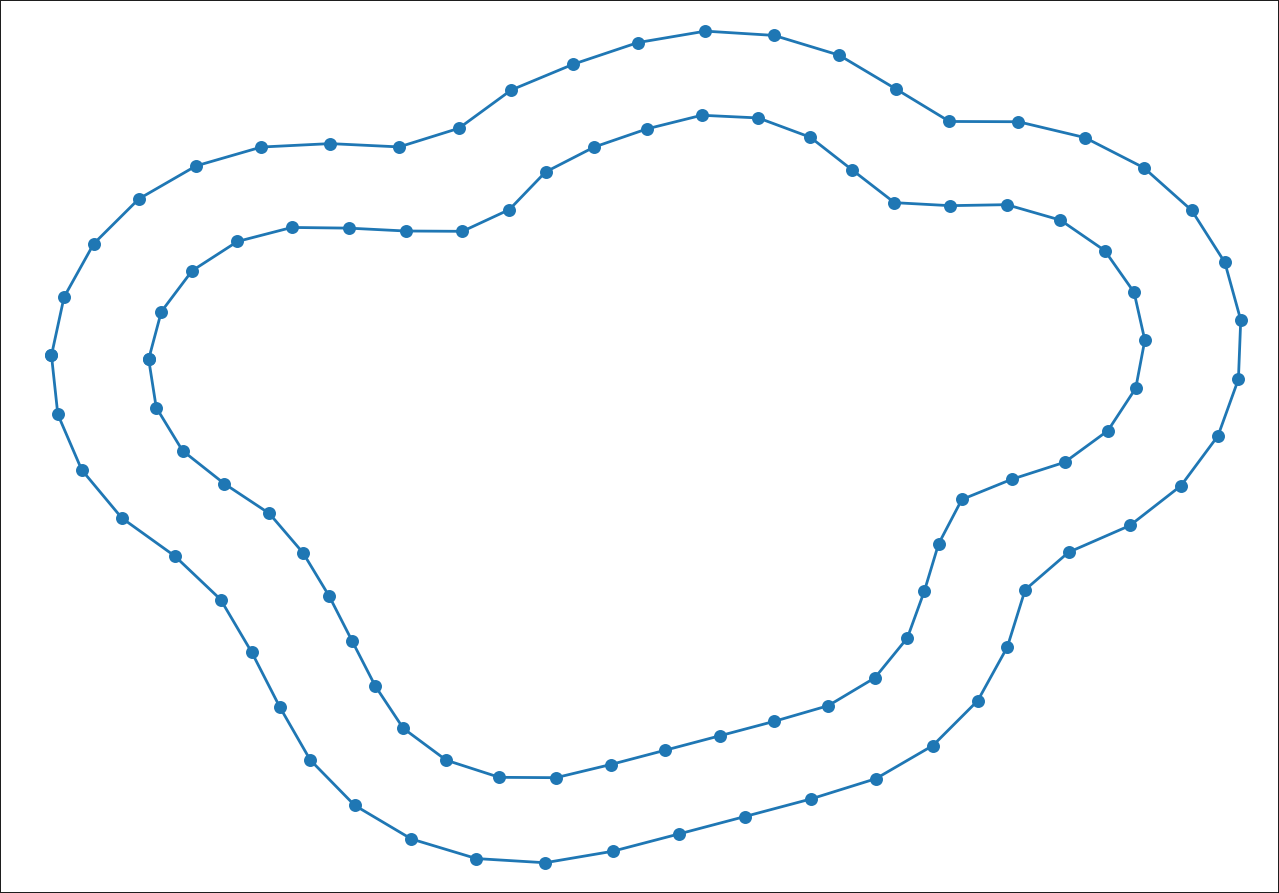
\includegraphics[width=\columnwidth]{track.png}}
\caption{The generated track boundaries using the RNG seed 42. Blue dots mark the positions of cones.}
\label{fig:track}
\end{center}
\vskip -0.2in
\end{figure}

\subsection{Gazebo ROS2 Communication}

Apart from system calls to interact with services provided by Gazebo Fortress we use the ROS-Gazebo-Bridge to convert the topics and data types published in Gazebo to ROS2. 
This is a transport layer that is available in python and can be launched using ROS2 and the regular python launch file syntax. 
This conversion process is very resource intensive which is why only the LiDAR sensor and the odometry can be updated with a high frequency.

